%===============================================================================
% LaTeX sjabloon voor de bachelorproef toegepaste informatica aan HOGENT
% Meer info op https://github.com/HoGentTIN/bachproef-latex-sjabloon
%===============================================================================

\documentclass{bachproef-tin}

\usepackage{hogent-thesis-titlepage} % Titelpagina conform aan HOGENT huisstijl

%%---------- Documenteigenschappen ---------------------------------------------
% TODO: Vul dit aan met je eigen info:

% De titel van het rapport/bachelorproef
\title{Wat is de meest performante manier om data te ontvangen en te verzenden op het web: Een vergelijkende studie tussen gRPC met Protocol Buffers en REST met JSON en proof-of-concept}

% Je eigen naam
\author{Sven Pepermans}

% De naam van je promotor (lector van de opleiding)
\promotor{Antonia Pierreux}

% De naam van je co-promotor. Als je promotor ook je opdrachtgever is en je
% dus ook inhoudelijk begeleidt (en enkel dan!), mag je dit leeg laten.
\copromotor{Kristof van Moorter}

% Indien je bachelorproef in opdracht van/in samenwerking met een bedrijf of
% externe organisatie geschreven is, geef je hier de naam. Zoniet laat je dit
% zoals het is.
\instelling{The Fashion Society}

% Academiejaar
\academiejaar{2020-2021}

% Examenperiode
%  - 1e semester = 1e examenperiode => 1
%  - 2e semester = 2e examenperiode => 2
%  - tweede zit  = 3e examenperiode => 3
\examenperiode{2}

%===============================================================================
% Inhoud document
%===============================================================================

\begin{document}

%---------- Taalselectie -------------------------------------------------------
% Als je je bachelorproef in het Engels schrijft, haal dan onderstaande regel
% uit commentaar. Let op: de tekst op de voorkaft blijft in het Nederlands, en
% dat is ook de bedoeling!

%\selectlanguage{english}

%---------- Titelblad ----------------------------------------------------------
\inserttitlepage

%---------- Samenvatting, voorwoord --------------------------------------------
\usechapterimagefalse
%%=============================================================================
%% Voorwoord
%%=============================================================================

\chapter*{\IfLanguageName{dutch}{Woord vooraf}{Preface}}
\label{ch:voorwoord}
Ik heb deze bachelorproef geschreven voor het voltooien van mijn opleiding Toegepaste Informatica met als afstudeerrichting Mobile Apps. Ik heb dit onderzoek rond performantie tussen gRPC met Protocol Buffers en REST met JSON voor de implementatie van The Fashion Society uitgevoerd omdat ik grote interesse heb in het ontwikkelen van back-end applicaties en services. Daarnaast vind ik de back-end structuur van de Fashion Society waarmee ik leren werken heb gedurende mijn stage zeer intrigerend en vond ik het passend om te onderzoeken of het systeem performanter te maken is door enkel het gebruikte dataformaat, en de bijhorende structuur, aan te passen.
Dit onderzoek heeft mij doen inzien dat er meer dan enkel REST en JSON is voor back-end applicaties en services. Waar ik voordien standaard JSON gebruikte zal ik nu eerst grondig nadenken of het niet beter is om een alternatief dataformaat te gebruiken.

Deze bacherlorproef zou echter niet tot stand zijn gekomen zijn zonder de hulp en bijstand van enkele mensen. Wat hierop volgt is een bedanking aan alle mensen die mij gesteund en geholpen hebben bij het ontwikkelen van deze bachelorproef.
 
Eerst en vooral zou ik de Fashion Society en specifiek Yoerick Lemmelijn willen bedanken voor het vertrouwen dat zij in mij hebben gestoken met het toegang verlenen tot de interne test server waarop een kopie van hun systeem draait en dewelke ook gebruik maakt van gevoelige data zoals klantgegevens. Als volgt wil ik zeer graag mijn co-promotor Kristof van Moorter bedanken. Dankzij zijn uitgebreide kennis van zowel het interne systeem van de Fashion Society als back-end applicaties, microservices en dataformaten is toch wel een groot deel van mijn bachelorproef en om specifiek te zijn mijn Proof-Of-Concept mogelijk gemaakt.

Alsook wil ik graag mijn promotor Antonia Pierreux bedanken voor de bijstand en feedback op de inhoud van deze bachelorproef, zij stond altijd klaar voor het verbeteren van een nieuwe toevoeging aan deze bachelorproef en hiervan had ik ook steeds snel de feedback, daarnaast wil ik haar ook bedanken voor het altijd klaar staan voor te antwoorden op soms, wat ik zelf kan beschrijven als domme, vragen.

Vervolgens zou ik ook mijn ouders, vriendin en vrienden willen bedanken voor mij te pushen op de momenten dat het nodig was zodanig dat deze bachelorproef voor de deadline zou afgeraakt zijn en om regelmatig mijn tussentijdse versies te proof readen.

Tot slot wil ik ook mijn medestudenten van campus Aalst bedanken voor de behulpzaamheid en alle verduidelijkingen die zij via de Discord server gegeven hebben in tijden van onzekerheid en onduidelijkheid.

Bij deze wens ik u een aangename leeservaring toe.
%% TODO:
%% Het voorwoord is het enige deel van de bachelorproef waar je vanuit je
%% eigen standpunt (``ik-vorm'') mag schrijven. Je kan hier bv. motiveren
%% waarom jij het onderwerp wil bespreken.
%% Vergeet ook niet te bedanken wie je geholpen/gesteund/... heeft


%%=============================================================================
%% Samenvatting
%%=============================================================================

% TODO: De "abstract" of samenvatting is een kernachtige (~ 1 blz. voor een
% thesis) synthese van het document.
%
% Deze aspecten moeten zeker aan bod komen:
% - Context: waarom is dit werk belangrijk?
% - Nood: waarom moest dit onderzocht worden?
% - Taak: wat heb je precies gedaan?
% - Object: wat staat in dit document geschreven?
% - Resultaat: wat was het resultaat?
% - Conclusie: wat is/zijn de belangrijkste conclusie(s)?
% - Perspectief: blijven er nog vragen open die in de toekomst nog kunnen
%    onderzocht worden? Wat is een mogelijk vervolg voor jouw onderzoek?
%
% LET OP! Een samenvatting is GEEN voorwoord!

%%---------- Nederlandse samenvatting -----------------------------------------
%
% TODO: Als je je bachelorproef in het Engels schrijft, moet je eerst een
% Nederlandse samenvatting invoegen. Haal daarvoor onderstaande code uit
% commentaar.
% Wie zijn bachelorproef in het Nederlands schrijft, kan dit negeren, de inhoud
% wordt niet in het document ingevoegd.

\IfLanguageName{english}{%
\selectlanguage{dutch}
\chapter*{Samenvatting}
\selectlanguage{english}
}{}

%%---------- Samenvatting -----------------------------------------------------
% De samenvatting in de hoofdtaal van het document

\chapter*{\IfLanguageName{dutch}{Samenvatting}{Abstract}}

Op basis van dit onderzoek kan The Fashion Society kiezen om de huidige structuur van de Discovery API, zijnde REST met JSON, te behouden of over te schakelen naar gRPC met Protocol Buffers. Dit onderzoek is interessant doordat The Fashion Society als maar blijft uitbreiden en er dagelijks honderdduizenden requests passeren door zowel de Orchestrator als de Discovery API en opmerkelijke verbeteringen in performantie door de eindgebruiker, zijnde het personeel van The Fashion Society en onderliggende bedrijven, duidelijk gevoeld kunnen worden. In dit onderzoek worden REST met JSON en gRPC met Protocol Buffers onderzocht en met elkaar vergeleken. Voor het uitvoeren van dit onderzoek wordt gebruik gemaakt van de testserver van The Fashion Society waar de huidige structuur reeds op geïmplementeerd is. De twee structuren worden vergeleken op basis van performantie in twee groeperingen, de kleine payload bestaande uit vierduizend requests en de grote payload bestaande uit veertigduizend requests. Verder in dit document zult u een inleiding tot het onderwerp vinden waarin onder andere de huidige stand van zaken, de onderzoeksvraag en het verdere verloop van deze bachelorproef beschreven staan. Alsook vindt u voor elk van beide structuren de resultaten van beide payloads.
%TODO Aanvullen met resultaat van onderzoek.

%---------- Inhoudstafel -------------------------------------------------------
\pagestyle{empty} % Geen hoofding
\tableofcontents  % Voeg de inhoudstafel toe
\cleardoublepage  % Zorg dat volgende hoofstuk op een oneven pagina begint
\pagestyle{fancy} % Zet hoofding opnieuw aan

%---------- Lijst figuren, afkortingen, ... ------------------------------------

% Indien gewenst kan je hier een lijst van figuren/tabellen opgeven. Geef in
% dat geval je figuren/tabellen altijd een korte beschrijving:
%
%  \caption[korte beschrijving]{uitgebreide beschrijving}
%
% De korte beschrijving wordt gebruikt voor deze lijst, de uitgebreide staat bij
% de figuur of tabel zelf.

\listoffigures
\listoftables

% Als je een lijst van afkortingen of termen wil toevoegen, dan hoort die
% hier thuis. Gebruik bijvoorbeeld de ``glossaries'' package.
% https://www.overleaf.com/learn/latex/Glossaries

%---------- Kern ---------------------------------------------------------------

% De eerste hoofdstukken van een bachelorproef zijn meestal een inleiding op
% het onderwerp, literatuurstudie en verantwoording methodologie.
% Aarzel niet om een meer beschrijvende titel aan deze hoofstukken te geven of
% om bijvoorbeeld de inleiding en/of stand van zaken over meerdere hoofdstukken
% te verspreiden!

%%=============================================================================
%% Inleiding
%%=============================================================================

\chapter{\IfLanguageName{dutch}{Inleiding}{Introduction}}
\label{ch:inleiding}

De inleiding moet de lezer net genoeg informatie verschaffen om het onderwerp te begrijpen en in te zien waarom de onderzoeksvraag de moeite waard is om te onderzoeken. In de inleiding ga je literatuurverwijzingen beperken, zodat de tekst vlot leesbaar blijft. Je kan de inleiding verder onderverdelen in secties als dit de tekst verduidelijkt. Zaken die aan bod kunnen komen in de inleiding~\autocite{Pollefliet2011}:

\begin{itemize}
  \item context, achtergrond
  \item afbakenen van het onderwerp
  \item verantwoording van het onderwerp, methodologie
  \item probleemstelling
  \item onderzoeksdoelstelling
  \item onderzoeksvraag
  \item \ldots
\end{itemize}

\section{\IfLanguageName{dutch}{Probleemstelling}{Problem Statement}}
\label{sec:probleemstelling}

Zoals eerder vermeld in deze bachelorproef is The Fashion Society constant aan het uitbreiden, dit onder andere door overnames en het openen van eigen nieuwe ZEB winkels. Elk van deze nieuwe winkels werkt via het centraal systeem en maakt dus onwetend gebruik van de Discovery API bij ondermeer het informeren van de stock, verkopen van een artikel, etc. Naarmate er meer winkels zijn zullen er ook meer gelijktijdige requests afgehandeld worden door de Discovery API. Door deze toename aan requests kan het al eens zijn dat de performantie daalt. Met dit onderzoek wordt hierop ingespeeld en wordt gekeken of gRPC met Protocol Buffers een performanter alternatief kan zijn op de huidige implementatie.

\section{\IfLanguageName{dutch}{Onderzoeksvraag}{Research question}}
\label{sec:onderzoeksvraag}

De onderzoeksvragen die gevormt worden bij de vergelijking tussen gRPC met Protocol Buffers en REST met JSON zullen dan ook zijn als volgt.
\begin{itemize}
    \item Welk dataformaat is het meest performant voor de Discovery API van The Fashion Society?
    \item Is gRPC met ProtocolBuffers sneller dan REST API met JSON voor de implementatie van The Fashion Society?
    \item Is gRPC met ProtocolBuffers efficiënter dan REST API met JSON voor de implementatie van The Fashion Society?
\end{itemize}

\section{\IfLanguageName{dutch}{Onderzoeksdoelstelling}{Research objective}}
\label{sec:onderzoeksdoelstelling}

Wat is het beoogde resultaat van je bachelorproef? Wat zijn de criteria voor succes? Beschrijf die zo concreet mogelijk. Gaat het bv. om een proof-of-concept, een prototype, een verslag met aanbevelingen, een vergelijkende studie, enz.

\section{\IfLanguageName{dutch}{Opzet van deze bachelorproef}{Structure of this bachelor thesis}}
\label{sec:opzet-bachelorproef}

% Het is gebruikelijk aan het einde van de inleiding een overzicht te
% geven van de opbouw van de rest van de tekst. Deze sectie bevat al een aanzet
% die je kan aanvullen/aanpassen in functie van je eigen tekst.

De rest van deze bachelorproef is als volgt opgebouwd:

In Hoofdstuk~\ref{ch:stand-van-zaken} wordt een overzicht gegeven van de stand van zaken binnen het onderzoeksdomein, op basis van een literatuurstudie.

In Hoofdstuk~\ref{ch:methodologie} wordt de methodologie toegelicht en worden de gebruikte onderzoekstechnieken besproken om een antwoord te kunnen formuleren op de onderzoeksvragen.

% TODO: Vul hier aan voor je eigen hoofstukken, één of twee zinnen per hoofdstuk

In Hoofdstuk~\ref{ch:conclusie}, tenslotte, wordt de conclusie gegeven en een antwoord geformuleerd op de onderzoeksvragen. Daarbij wordt ook een aanzet gegeven voor toekomstig onderzoek binnen dit domein.
\chapter{\IfLanguageName{dutch}{Stand van zaken}{State of the art}}
\label{ch:stand-van-zaken}

% Tip: Begin elk hoofdstuk met een paragraaf inleiding die beschrijft hoe
% dit hoofdstuk past binnen het geheel van de bachelorproef. Geef in het
% bijzonder aan wat de link is met het vorige en volgende hoofdstuk.

% Pas na deze inleidende paragraaf komt de eerste sectiehoofding.

In de inleiding is duidelijk geworden dat het onderzoek gericht zal zijn op twee mogelijke dataformaten aan de hand van 2 verschillende structuren, namelijk JSON aan de hand van REST en gRPC aan de hand van Protocol Buffers. Om dit onderzoek volledig te kunnen begrijpen is het belangrijk om de werking en de basisprincipes van deze dataformaten en de daarbij behorende structuren te begrijpen. Om deze reden zullen eerst de werking en basisprincipes van JSON en RESTful API worden uitgelegd, en als volgt die van gRPC en Protocol Buffers.

\section{JSON}
\label{sec:JSON}

\subsection{Algemeen}
\label{subsec:Algemeen}

JSON is een dataformaat zoals bijvoorbeeld XML en de afkorting staat voor JavaScript Object Notation. JSON is zoals beschreven in Standard ECMA-404 ~\autocite{Json2017} een dataformaat dat geïnspireerd is door de object constanten van JavaScript dat ook gekend staat als ECMAScript en is een structuur van accolades, haakjes, dubbele punten en komma's die zeer nuttig kunnen zijn in verschillende contexten, profielen en applicaties. Een voorbeeld hiervan is te zien in figuur \ref{fig:jsonExample}.

\begin{figure}[H]
    \centering
    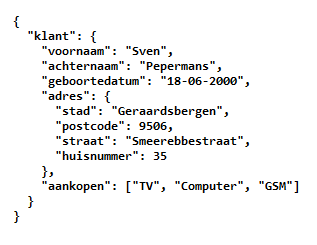
\includegraphics[scale=1.50]{jsonExample}
    \caption[JSON Example]{Een voorbeeld van een JSON.}
    \label{fig:jsonExample}
\end{figure}

JSON mag niet gezien worden als een specificatie van een gegevensuitwisseling want dat is het ook niet. Bij een zinvolle gegevensuitwisseling wordt er een overeenstemming over de structuur die gekoppeld is aan een gebruik van JSON tussen producent en consument vereist. JSON kan wel gezien worden als een syntactisch raamwerk waaraan een specifieke structuur kan worden gekoppeld.

Doordat er veel verschillende types getallen zijn zoals decimale en binaire getallen, kiest JSON enkel voor een weergave van getallen die mensen gebruiken, namelijk een reeks cijfers. Ook al zijn alle programmeertalen het niet altijd eens over de interne representaties van getallen, ze weten wel hoe ze cijferreeksen moeten begrijpen.

 Objecten kunnen op veel verschillende manieren voorgesteld worden, met andere woorden kunnen de modellen van objecten heel erg uiteenlopen. Om dit probleem aan te pakken biedt JSON een eenvoudige notatie aan voor het uitdrukken van verzamelingen met naam / waarde-paren. Om zulke verzamelingen weer te geven hebben de meeste programmeertalen reeds een functie zoals struct, map, hash en object.
Daarnaast biedt JSON ook ondersteuning voor geordende zoeklijsten, alsook hiervoor hebben alle programmeertalen een functie om deze weer te geven zoals array, vector en list. Aangezien objecten en arrays zich kunnen nesten, kunnen aan de hand van JSON complexe structuren zoals boomstructuren worden gerepresenteerd.

Hieruit kan worden geconcludeerd dat door het aanvaarden van JSON's simpele conventies, complexe datastructuren uitgewisseld kunnen worden tussen wat anders incompatiebele programmeertalen zijn.



\subsection{JSON in detail bekeken}
\label{subsec:JSON in detail bekeken}

Een JSON-tekst bestaat uit een reeks tokens die gevormd zijn uit Unicode-codepunten en die in overeenstemming zijn met de achterliggende JSON grammatica. Zo een reeks tokens bevat tekenreeksen, cijfers, zes structurele tokens en drie letterlijke naamtokens.
Hieronder volgt een opsomming van de zes structurele tokens en de drie literal name tokens.

De zes structurele tokens:

\begin{itemize}
    \item $\rbrack$ Linker vierkante haak
    \item $\rbrack$ Rechter vierkante haak
    \item \{ Linker accolade
    \item \} Rechter accolade
    \item : Dubbele punt
    \item , Komma
\end{itemize}

De drie literal name tokens:

\begin{itemize}
    \item true  
    \item false     
    \item null      
\end{itemize}

Voor of na de meeste tokens is het toegestaan om witruimte te gebruiken, echter niet in ze allemaal, een spatie is hierop een uitzondering en is wel toegestaan in strings. deze witruimte kan beschreven worden als een willekeurige reeks van één of meerdere van onderstaande codepunten.

\begin{itemize}
    \item Tekentabel       
    \item Regelinvoer       
    \item Regelterugloop   
    \item Spatie           
\end{itemize}


\subsection{Waarden}
\label{subsec:Waarden}

De bovengestelde tokens vormen de ruggengraat van een JSON-bestand, echter is het de bedoeling dat een JSON-bestand data overdraagt. Deze data kan aan de hand van verschillende waarden worden voorgesteld, namelijk als objecten, arrays, nummers, strings, true, false en null. Alle mogelijke waarden zijn zichtbaar in figuur \ref{jsonValue}.

\begin{figure}[ht]
    \centering
    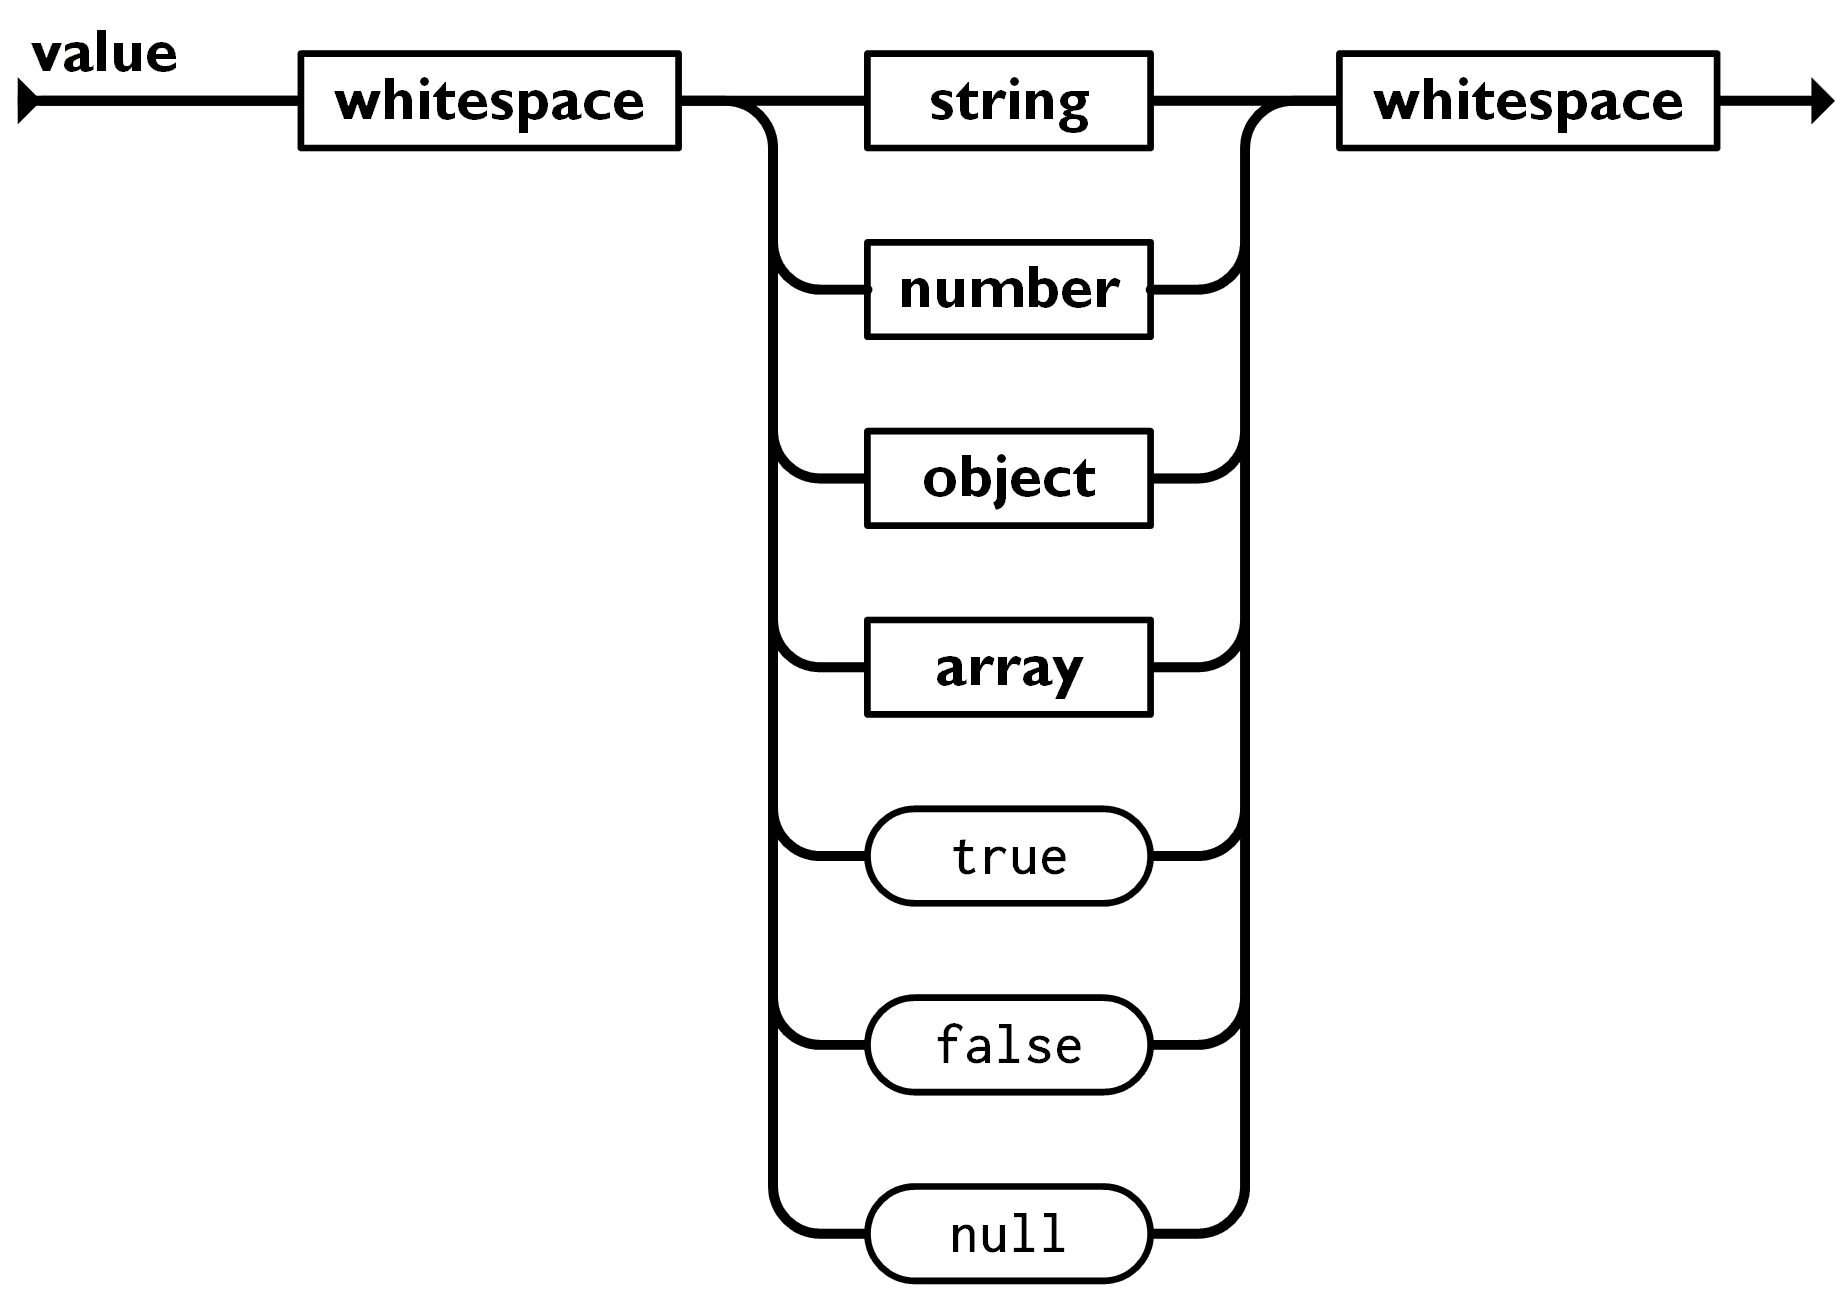
\includegraphics[scale=0.75]{jsonValue}
   \caption[JSON values]{De structuur van een JSON-waarde met alle mogelijke waarden die deze kan bevatten. Bron: \url{www.json.org}}
   \label{fig:jsonValue}
\end{figure}

De eerste waarden die besproken worden zijn de objecten, deze worden voorgesteld door een paar accolades die geen of meerdere name/value paren kunnen omringen zoals te zien is in figuur \ref{fig:jsonObject} en in figuur \ref{fig:objectEx}. In zo een name/value paar is de naam een string en wordt gevolgd door een dubbele punt die de naam en waarde van elkaar onderscheidt. 
Na de waarde kan optioneel een komma gezet worden, deze onderscheidt de waarde en de volgende naam van elkaar. Tot slot moeten de namen niet uniek zijn en moeten ze geen bepaalde ordening volgen.

\begin{figure}[H]
    \centering
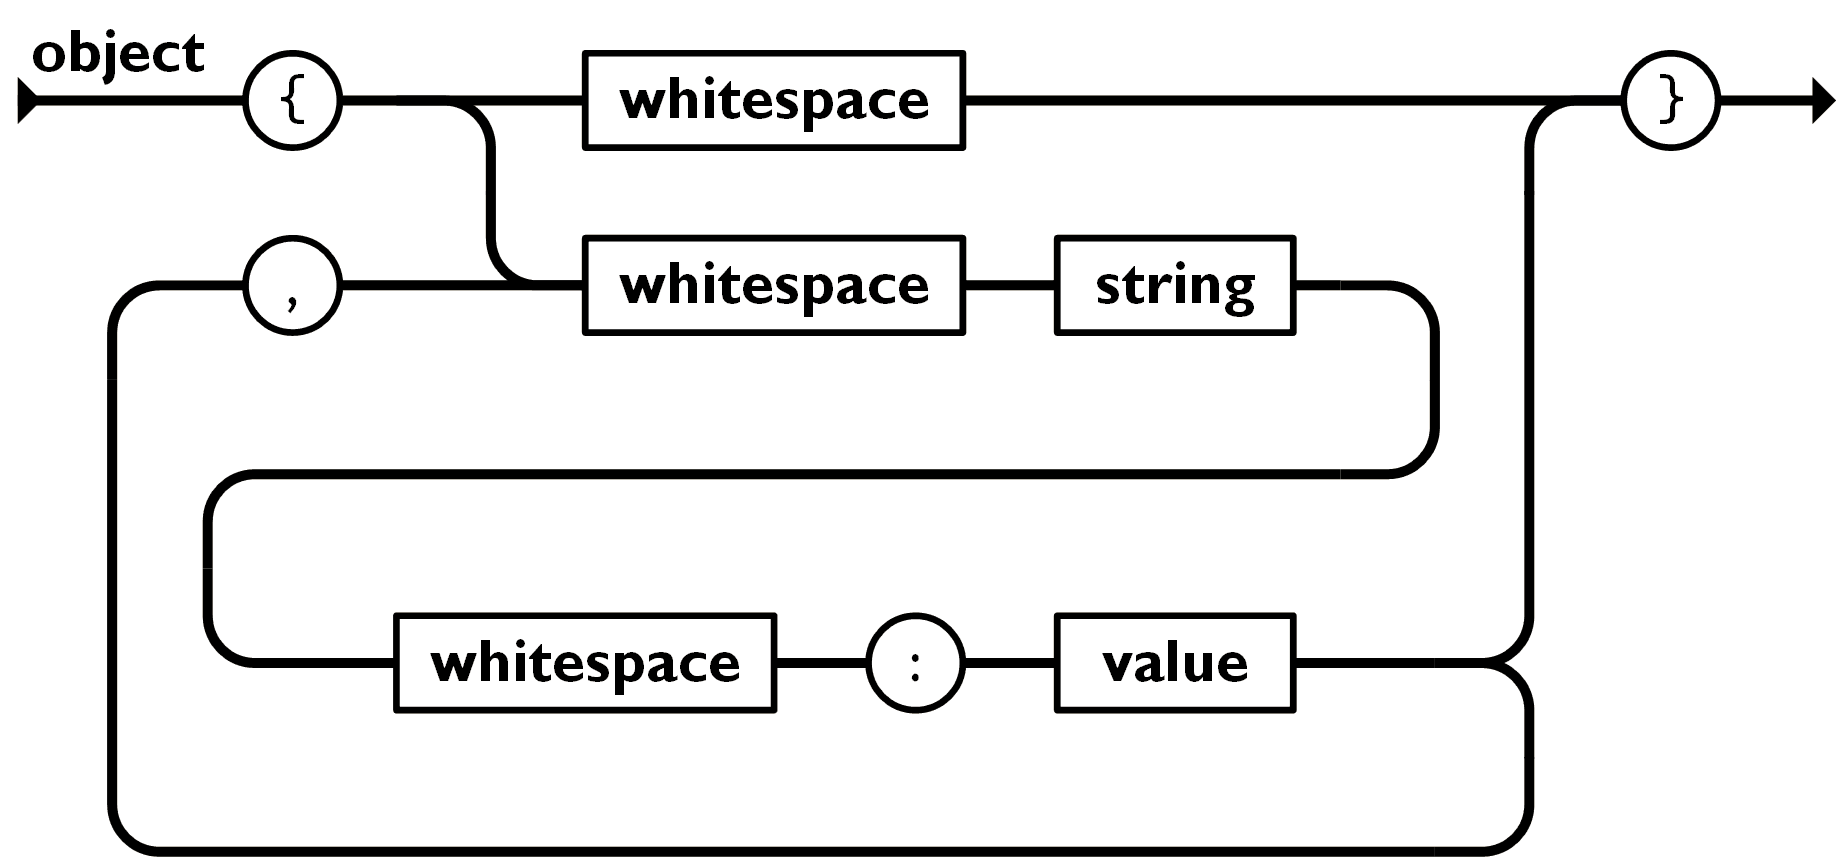
\includegraphics[scale=0.75]{jsonObject}
\caption[JSON Object Structuur]{De structuur van een JSON object. Bron: \url{www.json.org}}
    \label{fig:jsonObject}
\end{figure}

\begin{figure}[H]
    \centering
    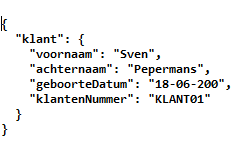
\includegraphics[scale=1.5]{objectEx}
    \caption[JSON Object]{Voorbeeld van een JSON object.}
    \label{fig:objectEx}
\end{figure}

Een tweede waarde zijn de arrays, dit zijn vierkante haken die geen of meerdere waarden omringen. Het bijzondere aan arrays is dat deze niet beperkt zijn tot een name/value paar en dus ook andere arrays kunnen bevatten en genest kunnen worden. Dit kan afgeleid worden uit figuur \ref{fig:jsonArray}. De array structuur wordt net zoals bij objecten geen beperkingen opgelegd, echter worden deze vooral gebruikt in situaties waar de ordening wel enig belang heeft. Figuur \ref{fig:arrayEx} is hier een duidelijk voorbeeld van.

\begin{figure}[H]
    \centering
    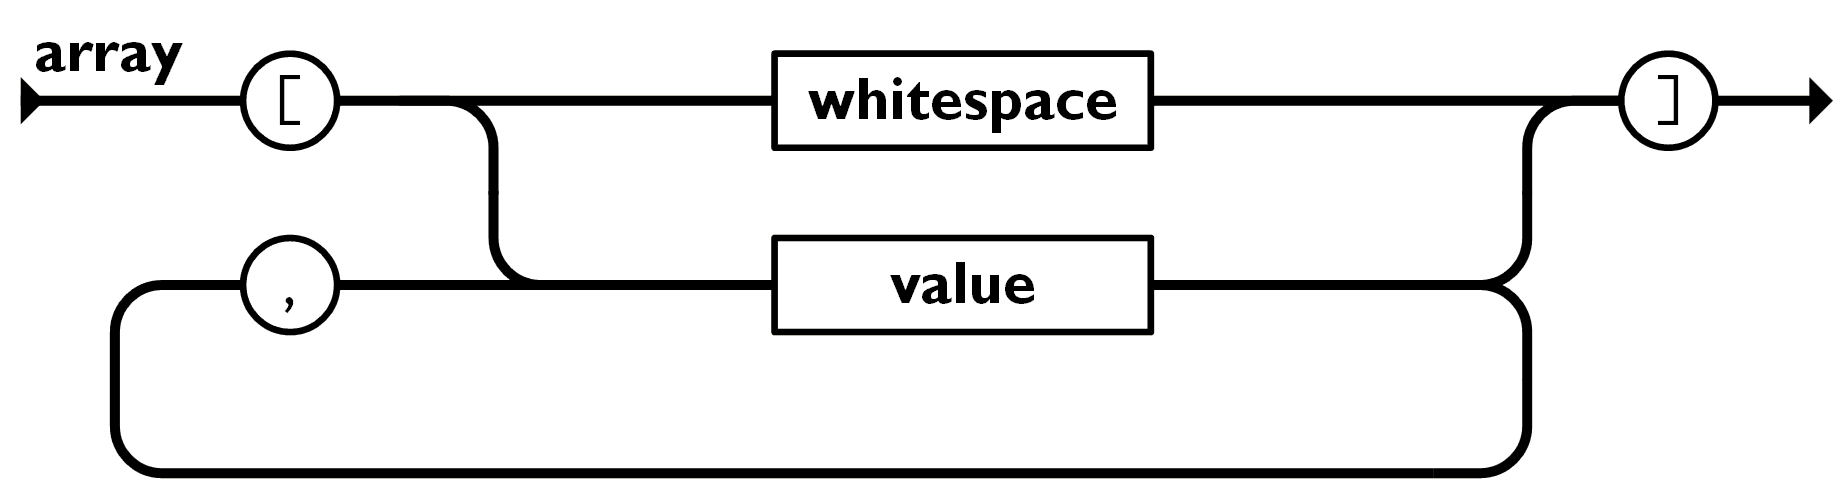
\includegraphics[scale=0.75]{jsonArray}
    \caption[JSON Array Structuur]{De structuur van een JSON array. Bron: \url{www.json.org}}
    \label{fig:jsonArray}
\end{figure}
\begin{figure}[H]
    \centering
    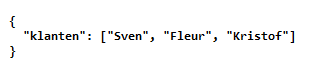
\includegraphics[scale=1.50]{arrayEx}
    \caption[JSON Array]{Een voorbeeld van een JSON Array.}
    \label{fig:arrayEx}
\end{figure}

Als volgt zijn er de nummers, een nummer kan gedefinieerd worden als een sequentie van decimale cijfers. Bij deze sequentie cijfers is er geen overbodige voorloopnul, een nummer kan wel voorafgegaan worden door een min-teken, als ook kan een nummer voorafgegaan worden door zowel een kleine als een grote e om een exponent aan te duiden dat  eventueel kan worden bijgestaan door een plus- of min-teken. Om te werken met kommagetallen wordt een decimaal punt gebruikt. Deze structuur is te zien in figuur \ref{fig:jsonNumber} en een voorbeeld hiervan in figuur \ref{fig:numberEx}.

\begin{figure}[H]
    \centering
    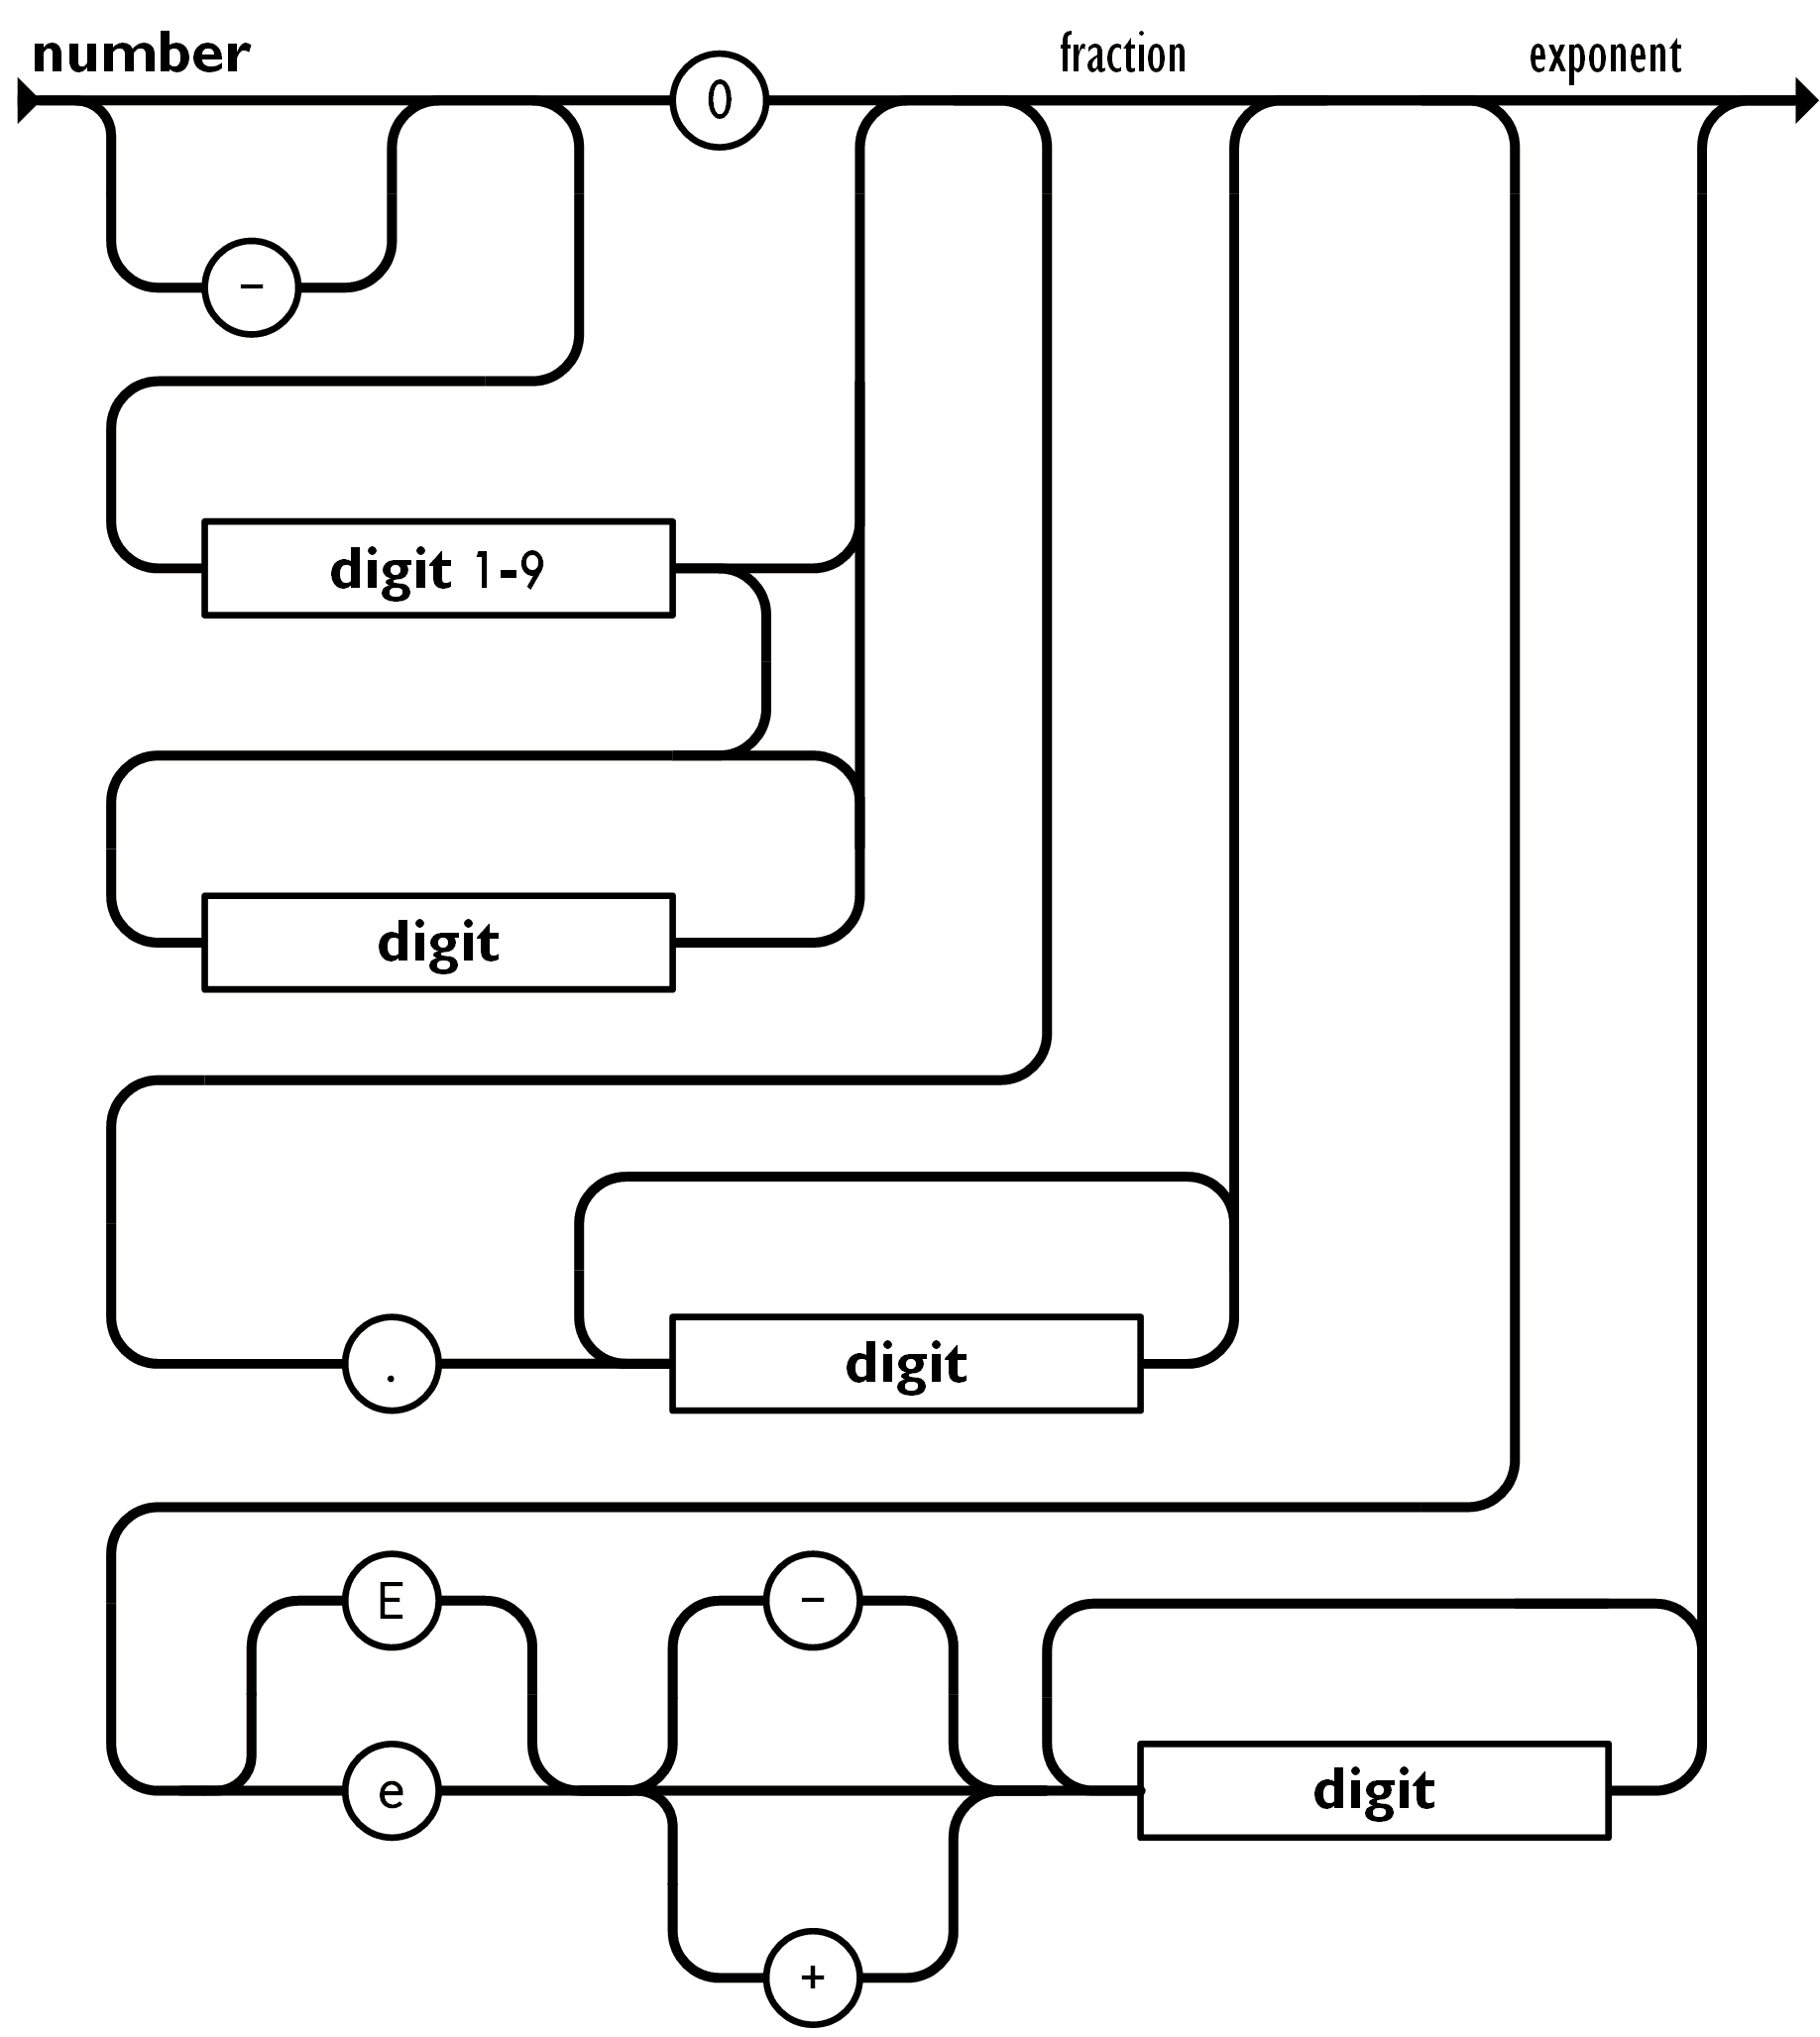
\includegraphics[scale=0.7]{jsonNumber}
    \caption[JSON Nummer Structuur]{De structuur van een JSON nummer. Bron: \url{www.json.org}}
    \label{fig:jsonNumber}
\end{figure}

\begin{figure}[H]
    \centering
    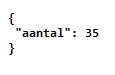
\includegraphics[scale=1.50]{numberEx}
    \caption[JSON Nummer]{Een voorbeeld van een JSON nummer.}
    \label{fig:numberEx}
\end{figure}

Tot slot zijn er de strings, deze representeren een tekst-waarde bestaande uit een sequentie van Unicode codepunten en zijn omringt door aanhalingstekens. Binnen deze aanhalingstekens zijn er echter enkele codepunten die niet gebruikt mogen worden, namelijk de karakters die moeten worden geëscaped. Dit zijn dan aanhalingstekens, backslash en de control karakters.
Voor sommige escape-reeksweergaven bestaande uit twee tekens bestaat er wel een representatie binnen de string, een representatie hiervan is te zien in \ref{fig:jsonString}.

Daarnaast kan ook elk codepunt weergegeven worden als een hexadecimale sequentie, waarvan de betekenis is vastgelegd in ISO/IEC 10646. Hexadecimale getallen kunnen zowel cijfers als kleine letters en hoofdletters van A tot F zijn.
De codepunten die zich bevinden in het Basic Multilingual Plane kunnen gerepresenteerd worden als een sequentie van zes karakters, namelijk een backslash gevolgd door een kleine letter u, en tot slot gevolgd door vier hexadecimale getallen die een codepunt encoderen. In figuur \ref{fig:jsonString} is de structuur van een string te zien.

\begin{figure}[H]
    \centering
    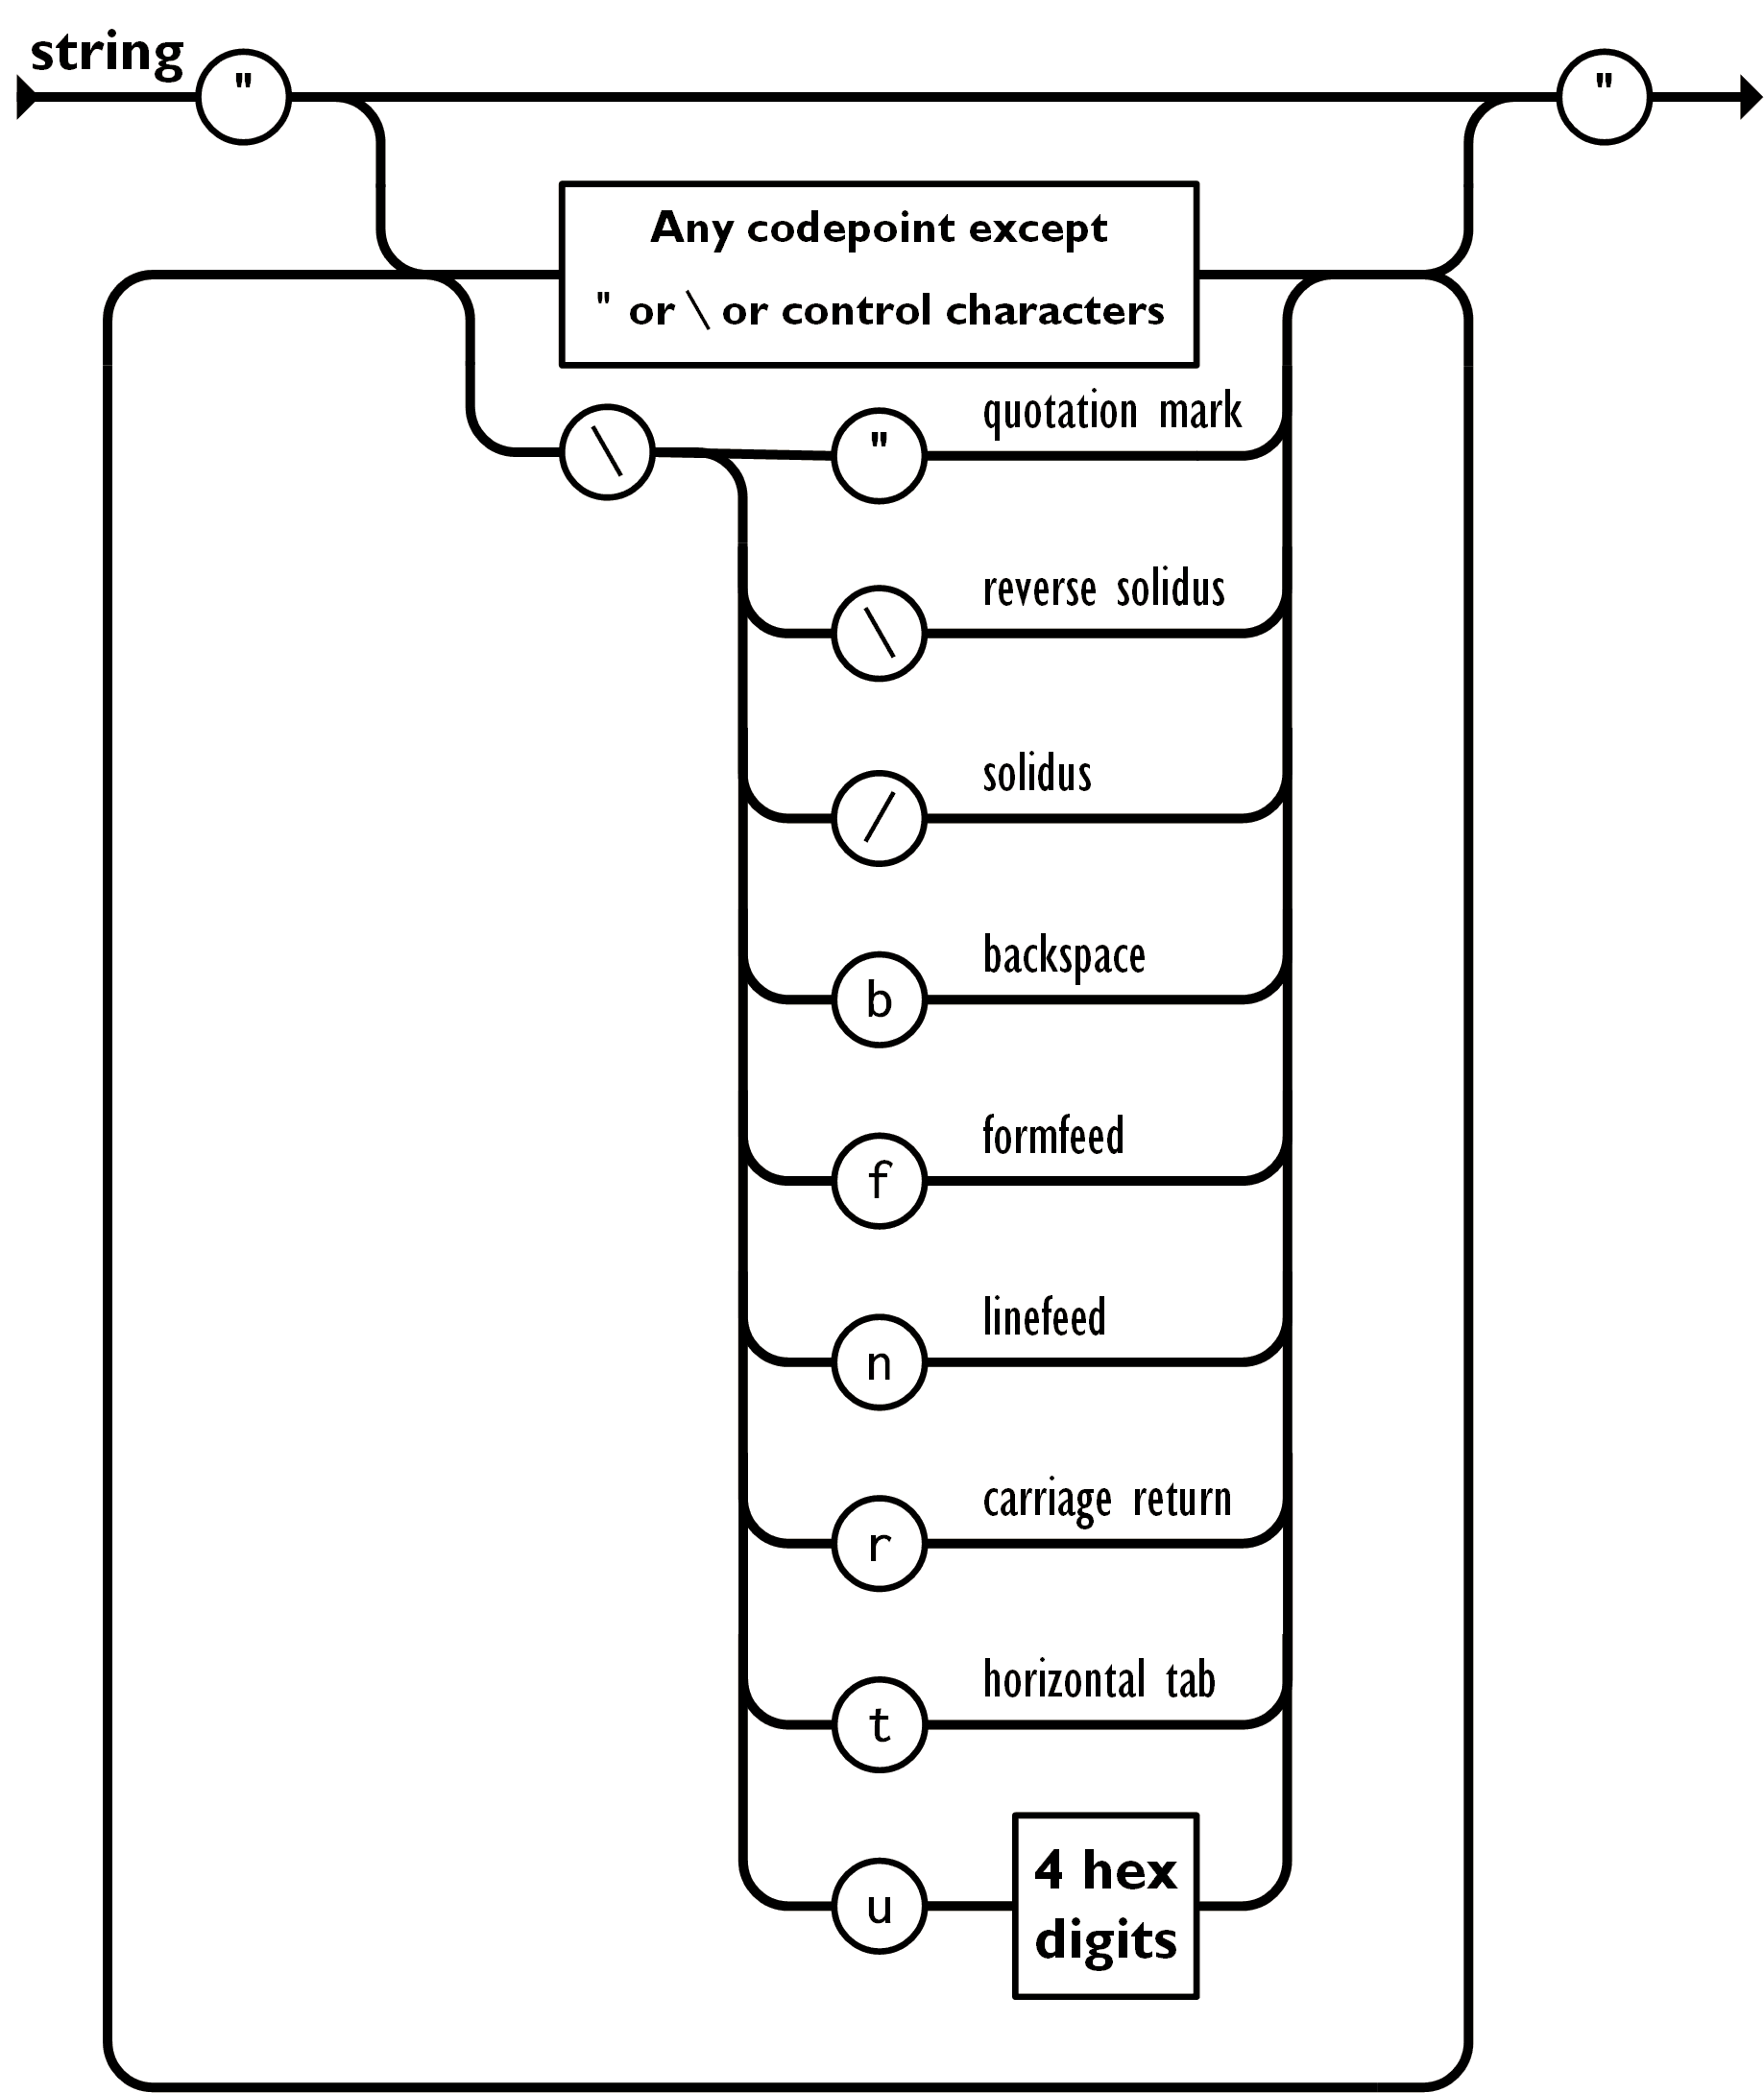
\includegraphics[scale=0.75]{jsonString}
    \caption[JSON String]{De structuur van een JSON string. Bron: \url{www.json.org}}
    \label{fig:jsonString}
\end{figure}


\section{RESTful API}
\label{sec:RESTful API}

Representational State Transfer (REST) is zoals beschreven door \textcite{Fielding2000} een architecturale stijl voor het ontwerpen van gedistribueerde hypermediasystemen.
Een Application Program Interface (API) is een lijst van regels of restricties die ervoor zorgen dat verschillende programma's met elkaar kunnen communiceren. \autocite{Hubspire}

De combinatie van REST en API is een RESTful API, wanneer een RESTful API gecalled wordt dan zal de server een representatie van de huidige staat van de gevraagde resource weergeven.

\subsection{Design principes}
\label{subsec:Design principes}

Om een API als RESTful te kunnen beschrijven moet deze voldoen aan zes design principes die hieronder zullen worden verduidelijkt aan de hand van \autocite{Long} en \autocite{Naeem2021}

\textbf{Client-Server}

Dit principe zegt dat zowel de client als de server apart moeten kunnen worden ontwikkeld en moeten los staan van elkaar. Op deze manier wordt de handelbaarheid en schaalbaarheid aanzienlijk verbetered aangezien de gebruikersinterface los staat van de gegevensopslag.


\textbf{Stateless}

Met stateless wordt bedoeld dat elke request die er naar de API gedaan wordt onafhankelijk is van elkaar, een request heeft dus geen resultaat nodig van een andere request om te kunnen verder gaan. Met andere woorden moet de server geen vorige requests en states opslaan wat de benaming 'Stateless' verklaard.


\textbf{Cacheable}

Een REST API moet de mogelijkheid hebben om data te cachen, dit is het opslaan van data in digitaal geheugen. Volgens het Cacheable principe moet data in een response al dien niet duidelijk gecategoriseerd worden als cacheable of non-cacheable. Indien een response cacheable is dan mag de cliënt cache deze data opslaan voor gelijkaardige requests in de toekomst te beantwoorden.

\textbf{Uniform interface}

Voor aan het client-server principe te voldoen is een uniforme interface nodig die autonome ontwikkeling van de applicatie mogelijk maakt zonder de acties, modellen en services te koppelen aan de API-laag. Door dit principe wordt de hele architectuur gestroomlijnd en wordt de visibiliteit van de communicatie verbeterd. Er zijn echter wel verschillende architecturale controles nodig die de performantie binnen de architectuur sturen om een uniforme interface te bereiken.

REST bevat vier interfacecontroles, namelijk: 

\begin{enumerate}
\item Identificatie van bronnen: Een Uniform Resource Locator (URL) identificeerd de online locatie van een resource.
\item Beheer van bronnen door middel van representatie: Bronnen worden weergegeven aan de hand van media types ~\autocite{N.Freed1996} zoals JSON en XML.
\item Zelfbeschrijvende communicatie: Een bericht bevat alle informatie die de ontvanger nodig heeft om de informatie te begrijpen. Er mag geen extra informatie in een aparte documentatie of apart bericht zitten. Deze zelfbeschrijvende communicatie gebeurd door het gebruik van de accept en content-type HTTP headers die de inhoud die verzonden of aangevraagd wordt beschrijft.
\item Hypermedia: Hypermedia is data dat verzonden wordt van de server naar de cliënt met informatie over wat de cliënt vervolgens kan doen. Hyper Text Markup Language (HTML) ~\autocite{W3schools} is hier een voorbeeld van.
\end{enumerate}
\textbf{Layered system}

De architectuur van een RESTful API bestaat uit verschillende lagen die door samen te werken een hiërarchie vormen die helpt bij het vormen van een flexibele, meer schaalbare applicatie. Dankzij het deze gelaagde structuur is de gevormde applicatie beter beveiligd, dit komt doordat componenten niet kunnen interageren buiten de eigen laag en de volgende laag. Daarnaast biedt het gedeelde caches aan die de schaalbaarheid verbeteren.

Deze gelaagde architectuur zorgt tot slot voor meer stabiliteit doordat het de componenten beperkt zodanig dat een component niet verder kan 'zien' als de laag waarmee het interageerd.

\textbf{Code on demand}

Het 'Code on demand' principe zorgt ervoor dat codering kan worden gecommuniceerd via de API voor gebruik binnen de applicatie. De definitie van een RESTful API maakt het mogelijk dat functionaliteit aan de cliënt-kant kan worden uitgebreid door codering zoals applets of scripts te downloaden en te implementeren. Dit stroomlijnt cliënts door het aantal functies te verminderen die vooraf moeten worden geïmplementeerd.

Naast statische resources zoals XML en JSON kan dus ook uitvoerbare code aangeleverd worden door de server.

\textbf{Resources}

Bij REST kan elk stuk informatie een resource zijn, dit kan van alles zijn zoals documenten, services, collecties van andere resources, afbeeldingen, en dergelijke. In sommige gevallen wordt “Everything as a resource”  een zevende principe van REST genoemd. 

\subsection{Hoe werkt een RESTful API?}
\label{subsec:Hoe werkt een RESTful API?}

Zoals eerder vermeld in subsectie \ref{subsec:Design principes} heeft elke resource een unieke URL, zo een URL wordt een request genoemd waarbij de gereturnde data gekend staat als een response. In een RESTful API worden deze requests of transacties in vier componenten verdeeld zoals uitgelegd in \autocite{Karine2020}.

\begin{itemize}
    \item \textbf{GET}: Deze request haalt een representatie van een resource op.
    \item \textbf{PUT}: Met PUT wordt een bestaande resource geupdatet.
    \item \textbf{POST}: Aan de hand van POST kunnen nieuwe resources en sub-resources aangemaakt worden.
    \item \textbf{DELETE}: De DELETE request gaat een reeds bestaande resource verwijderen.
\end{itemize}





%%=============================================================================
%% Methodologie
%%=============================================================================

\chapter{\IfLanguageName{dutch}{Praktijk onderzoek}{Practical Research}}
\label{ch:Praktijk onderzoek}

%% TODO: Hoe ben je te werk gegaan? Verdeel je onderzoek in grote fasen, en
%% licht in elke fase toe welke stappen je gevolgd hebt. Verantwoord waarom je
%% op deze manier te werk gegaan bent. Je moet kunnen aantonen dat je de best
%% mogelijke manier toegepast hebt om een antwoord te vinden op de
%% onderzoeksvraag.

In hoofdstuk 2 is het onderzoek gestart met een literatuurstudie waarin besproken werd wat REST, JSON, gRPC en Protobufs exact zijn en hoe de interne architectuur van Fashion Society er uitziet.

In dit hoofdstuk gaat het onderzoek verder met een requirementanalyse en een plan van aanpak waarin beschreven wordt hoe de proof-of-concept tot stand komt en wat de resultaten hiervan zijn.

\section{Requirementanalyse}
\label{sec:Requirementanalyse}

In deze analyse worden de functionele en niet-functionele vereisten opgelijst waaraan een alternatieve implementatie van de Discovery API moet voldoen.

Functionele requirements:
\begin{itemize}
    \item Implementatie aan de hand van .NET Core 3.1 voor long-term support.
    \item Moet een grote hoeveelheid aan parallelle requests kunnen afhandelen.

\end{itemize}

Niet-functionele requirements:
\begin{itemize}
    \item Moet (relatief) gemakkelijk uitbreidbaar zijn.
 \item Moet snel requests kunnen afhandelen.
     \item Moet schaalbaar zijn.
\end{itemize}



\section{Plan van aanpak}
\label{sec:Plan van aanpak}

\subsection{Opstellen van gRPC service in .NET Core 3.1 }
\label{subsec:Opstellen van gRPC service in .NET Core 3.1}
Uit de requirementanalyse kan afgeleid worden dat de service zal moeten draaien in .NET Core 3.1 en niet in .NET Core 5.0 omdat deze geen long-term support heeft van Microsoft.

Zodanig dat gebruik gemaakt kan worden van de voordelen van gRPC zoals codegeneratie zal het project opgebouwd worden vanuit een grpc service project vanuit Visual Studio zelf, dit project bevat de Grpc.AspNetCore package die alles gRPC gerelateerd afhandelt.

Voor de logica in de twee endpoints GetService en GetServiceUrl die respectievelijk een service object en een service url ophalen zal code gerecupereerd worden van de reeds bestaande Discovery API.

De reeds bestaande Discovery API maakt gebruik van het repository patroon voor het ophalen en verwerken van data uit een SQL database in de gRPC service zal dit patroon wegvallen en zal de databasecontext rechtstreeks in de Service geïnjecteerd worden. Uit een verdere analyse van de bestaande code kan er ook geconcludeerd worden dat beide methoden gebruik maken van éénzelfde Get methode in de repository, deze wordt een private methode in de Service die zal worden aangesproken door beide endpoints.

Het protobestand “services.proto” waaruit de bijhorende modellen worden gegenereerd bevat de 2 rpc methodes GetService en GetServiceUrl, beiden hebben deze een input parameter van het messagetype “ServiceName” met als veld een string “name”.
De GetService methode zal een message van het type “ServiceObject” teruggeven, deze bevat de “name”, “address”, “port”, “addNameToUrl” en “hasSwaggerDoc” velden. Deze velden zijn licht afwijkend van het reeds bestaande Model in de Discovery API maar is in samenspraak met mijn co-promotor.
Tot slot is er de GetServiceUrl methode, deze geeft een message van het type “ServiceUrl” terug dewelke een enkel veld bevat zijnde “url”.

In figuur \ref{fig:ProtoPoC} is het gebruikte protobestand te zien.

\begin{figure}[H]
    \centering
    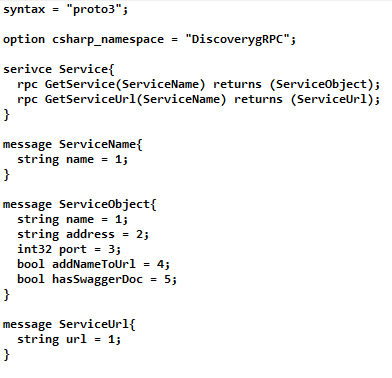
\includegraphics[scale=0.75]{ProtoPoC}
    \caption[Proof-Of-Concept protobestand]{Het gebruikte protobestand}
    \label{fig:ProtoPoC}
\end{figure}

\subsection{Client applicaties voor REST en gRPC}
\label{subsec:Client applicaties voor REST en gRPC}

Om de snelheid van beide implementaties te testen moeten de services worden aangesproken van een client. Hiervoor worden twee identieke implementaties gebruikt in twee Console applicaties (.NET Core). De enige verschillen tussen de twee applicaties zijn de aangesproken endpoints. Deze applicaties zullen aan de hand van een lijst van vier servicenamen calls doen naar de service. Er is voor vier servicenamen gekozen zodanig dat er rekening wordt gehouden met eventuele verschillen in het ophalen van de verschillende data.

Tijdens het gehele proces zal een timer lopen die de totale tijd van de calls zal opnemen.

\subsection{Het verloop van het onderzoek}
\label{subsec:Het verloop van het onderzoek}

Het onderzoek wordt uitgevoerd in drie categorieën, een kleine en grote payload voor het resultaat van parallele requests en een request loop van tienduizend requests voor de response time voor één request te berekenen. In de kleine payload zullen er in totaal vierduizend calls gemaakt worden, elke servicenaam zal tien keer parallel gebruikt worden om vervolgens honderd requests te versturen. In de grote payload zullen er tienduizend calls gemaakt worden en hier zal elke servicenaam vijfentwintig keer parallel gebruikt worden om vervolgens honderd requests te versturen.

Om tot een concreet resultaat van één request te bekomen zal ook deze tienduizend keer worden uitgevoerd. Dit hoge aantal is gekozen om de invloed van eventuele netwerk vertragingen te beperken.
De kleine en grote payload zullen daarintegen vier keer uitgevoerd worden om tot een concreet resultaat te bekomen. Hier zullen eventuele netwerk vertragingen om individuele calls minder doorwegen door het reeds hoge aantal calls in elke uitvoering.


Het CPU gebruik zal manueel in de gaten gehouden worden maar zal in samenspraak met de co-promotor niet in acht genomen worden in de resultaten omdat er geen accurate manier beschikbaar is om het CPU gebruik op de server te registreren.

\section{Resultaat Proof-Of-Concept}
\label{sec:Resultaat Proof-Of-Concept}

\subsection{Single Call}
\label{subsec:Single Call}
Uit het onderzoek is gebleken dat gRPC met ProtocolBuffers voor zowel de GetService methode (-24,06\%) als de GetServiceUrl methode (-23,78\%) sneller is dan REST met JSON.
\begin{figure}[H]
    \centering
    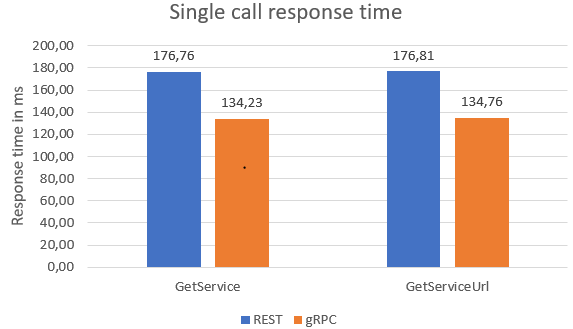
\includegraphics[scale=1]{singleCall}
    \caption[Single Call Response Time]{Resultaat van het onderzoek naar Single call response time.}
    \label{fig:SingleCallResult}
\end{figure}

De verwachting van dit onderdeel was dat het resultaat bij de single call response time een marginaal verschil ging zijn in voordeel van gRPC doordat de response op de calls een kleine hoeveelheid data is voor beide methodes, echter toonde het resultaat een groter dan verwacht verschil in snelheid in voordeel van gRPC.

\subsection{Vierduizend Parallelle Calls}
\label{subsec:Vierduizend parallelle calls}
Uit het onderzoek is gebleken dat gRPC voor zowel de GetService methode (-15,63\%) als voor de GetServiceUrl methode (-20,34\%) sneller is dan REST bij het afhandelen van vierduizend parallelle calls.
\begin{figure}[H]
    \centering
    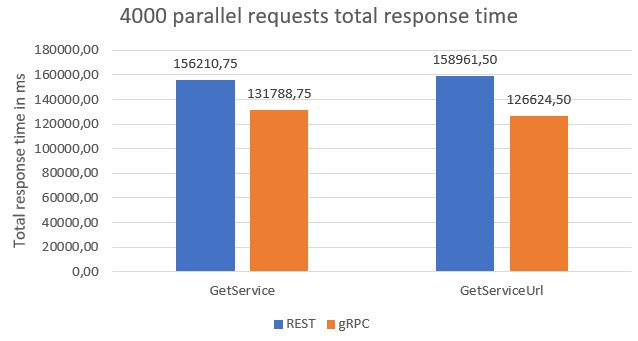
\includegraphics[scale=1]{VierduizendCalls}
    \caption[Resultaten van vierduizend parallelle calls]{Resultaat van het onderzoek naar een kleine hoeveelheid parallelle calls.}
    \label{fig:VierduizendCallsResult}
\end{figure}

Bij dit onderdeel is het resultaat onder de verwachtingen, de verwachtingen waren dat gRPC opmerkelijk sneller ging zijn dan REST door de hoeveelheid aan af te handelen requests. Echter is het gebleken dat dit een verkeerde redenering was voor de verwachting, de hoeveelheid data in de response op elke call blijft namelijk nog altijd klein.

\subsection{Tienduizend Parallelle Calls}
\label{subsec:Tienduizend parallelle calls}
Uit het onderzoek is gebleken dat gRPC voor zowel de GetService methode (-13,96\%) als voor de GetServiceUrl methode (-16,35\%) sneller is dan REST bij het afhandelen van tienduizend parallelle calls.
\begin{figure}[H]
    \centering
    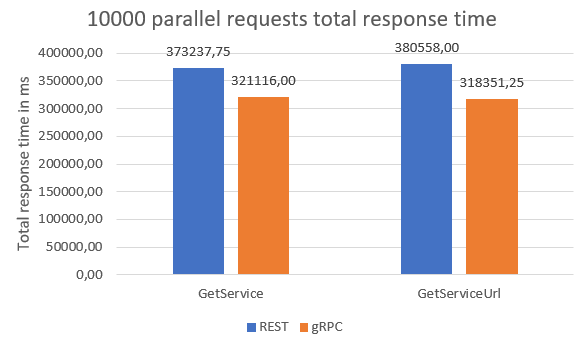
\includegraphics[scale=1]{TienduizendCalls}
    \caption[Resultaten van tienduizend parallelle calls]{Resultaat van het onderzoek naar een grote hoeveelheid parallelle calls.}
    \label{fig:TienduizendCallsResult}
\end{figure}

Net zoals bij de kleine hoeveelheid parallelle calls is het resultaat hier onder de verwachtingen. gRPC is voor zowel de GetService methode (-13,96\%) als voor de GetServiceUrl methode (-16,35\%) sneller dan REST maar ook hier is voor de verwachting dezelfde verkeerde redenering gebruikt als bij de kleine hoeveelheid parallelle calls. Het aantal parallelle calls is wel verhoogd maar de hoeveelheid data in de response op de calls blijft nog altijd hetzelfde.



% Voeg hier je eigen hoofdstukken toe die de ``corpus'' van je bachelorproef
% vormen. De structuur en titels hangen af van je eigen onderzoek. Je kan bv.
% elke fase in je onderzoek in een apart hoofdstuk bespreken.

%\input{...}
%\input{...}
%...

%%=============================================================================
%% Conclusie
%%=============================================================================

\chapter{Conclusie}
\label{ch:conclusie}

% TODO: Trek een duidelijke conclusie, in de vorm van een antwoord op de
% onderzoeksvra(a)g(en). Wat was jouw bijdrage aan het onderzoeksdomein en
% hoe biedt dit meerwaarde aan het vakgebied/doelgroep? 
% Reflecteer kritisch over het resultaat. In Engelse teksten wordt deze sectie
% ``Discussion'' genoemd. Had je deze uitkomst verwacht? Zijn er zaken die nog
% niet duidelijk zijn?
% Heeft het onderzoek geleid tot nieuwe vragen die uitnodigen tot verder 
%onderzoek?

De opzet van dit onderzoek is om een antwoord te geven op de onderzoeksvragen “Welk dataformaat is performanter voor de Discovery API van de Fashion Society?”, “Is gRPC met ProtocolBuffers sneller dan REST API met JSON voor de implementatie van de Fashion Society?” en “Is gRPC met ProtocolBuffers efficiënter dan REST API met JSON op gebied van CPU gebruik voor de implementatie van de Fashion Society?”.
De conclusie is afhankelijk van de drie uitgevoerde testen, single call response time, totale response tijd voor vierduizend parallelle calls en totale response tijd voor tienduizend parallelle calls, die voor de methode GetService en GetServiceUrl zijn uitgevoerd.

\section{Single Call}
\label{sec:Single Call}
Uit het onderzoek is gebleken dat gRPC met ProtocolBuffers voor zowel de GetService methode (-24,06\%) als de GetServiceUrl methode (-23,78\%) sneller is dan REST met JSON.
\begin{figure}[H]
    \centering
    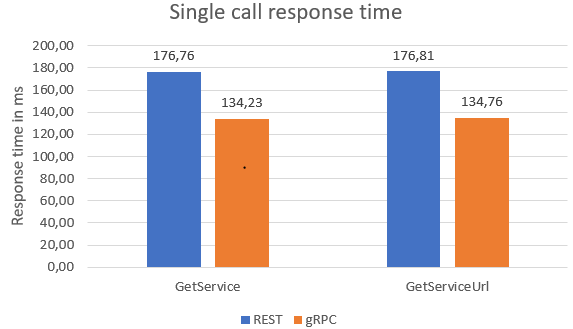
\includegraphics[scale=1]{singleCall}
    \caption[Single Call Response Time]{Resultaat van het onderzoek naar Single call response time.}
    \label{fig:SingleCallResult}
\end{figure}

De verwachting van dit onderdeel was dat het resultaat bij de single call response time een marginaal verschil ging zijn in voordeel van gRPC doordat de response op de calls een kleine hoeveelheid data is voor beide methodes, echter toonde het resultaat een groter dan verwacht verschil in snelheid in voordeel  van gRPC.

\section{Vierduizend Parallelle Calls}
\label{sec:Vierduizend parallelle calls}
Uit het onderzoek is gebleken dat gRPC voor zowel de GetService methode (-15,63\%) als voor de GetServiceUrl methode (-20,34\%) sneller is dan REST bij het afhandelen van vierduizend parallelle calls.
\begin{figure}[H]
    \centering
    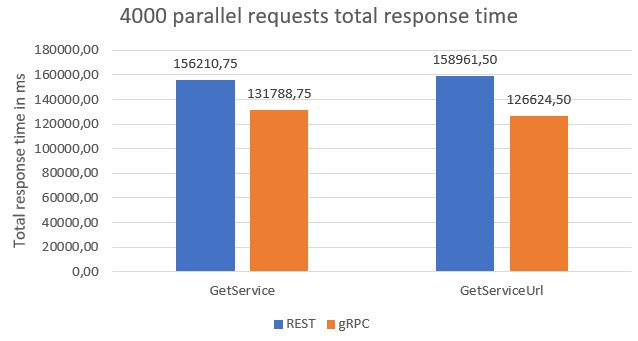
\includegraphics[scale=1]{VierduizendCalls}
    \caption[Resultaten van vierduizend parallelle calls]{Resultaat van het onderzoek naar een kleine hoeveelheid parallelle calls.}
    \label{fig:VierduizendCallsResult}
\end{figure}

Bij dit onderdeel is het resultaat onder de verwachtingen, de verwachtingen waren dat gRPC opmerkelijk sneller ging zijn dan REST door de hoeveelheid aan af te handelen requests. Echter is het gebleken dat dit een verkeerde redenering was voor de verwachting, de hoeveelheid data in de response op elke call blijft namelijk nog altijd klein.

\section{Tienduizend Parallelle Calls}
\label{sec:Tienduizend parallelle calls}
Uit het onderzoek is gebleken dat gRPC voor zowel de GetService methode (-13,96\%) als voor de GetServiceUrl methode (-16,35\%) sneller is dan REST bij het afhandelen van tienduizend parallelle calls.
\begin{figure}[H]
    \centering
    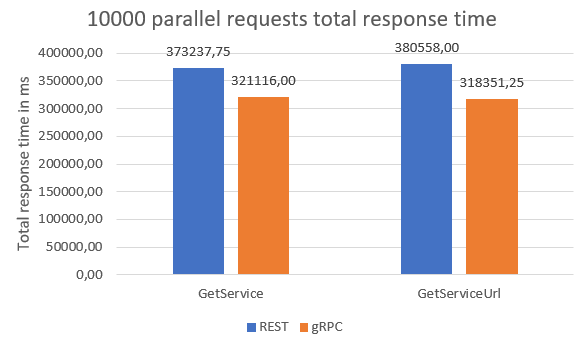
\includegraphics[scale=1]{TienduizendCalls}
    \caption[Resultaten van tienduizend parallelle calls]{Resultaat van het onderzoek naar een grote hoeveelheid parallelle calls.}
    \label{fig:TienduizendCallsResult}
\end{figure}

Net zoals bij de kleine hoeveelheid parallelle calls is het resultaat hier onder de verwachtingen. gRPC is voor zowel de GetService methode (-13,96\%) als voor de GetServiceUrl methode (-16,35\%) sneller dan REST maar ook hier is voor de verwachting dezelfde verkeerde redenering gebruikt als bij de kleine hoeveelheid parallelle calls. Het aantal parallelle calls is wel verhoogd maar de hoeveelheid data in de response op de calls blijft nog altijd hetzelfde.

\section{Besluit}
\label{sec:Besluit}

Uit het onderzoek kunnen twee van de drie onderzoeksvragen beantwoord worden. Er kan geconcludeerd worden dat gRPC met ProtocolBuffers sneller is dan REST met JSON voor de implementatie van The Fasion Society en dat ProtocolBuffers performanter zijn dan JSON voor de implementatie van de Fashion Society.

Op de onderzoeksvraag “Is gRPC met ProtocolBuffers efficiënter dan REST API met JSON op gebied van CPU gebruik voor de implementatie van de Fashion Society?” kan geen besluitend antwoord gegeven worden omdat deze gegevens niet exact meetbaar waren gedurende het uitvoeren van de proof-of-concept. Hierbij is in overleg met de co-promotor het besluit gevormd dat de Fashion Society een snel groeiend bedrijf is waarbij performantie belangrijk is en dat als er meer CPU gebruik zou zijn dit een prijs is dat het bedrijf gewillig is om te betalen in ruil voor een performantere implementatie.







%%=============================================================================
%% Bijlagen
%%=============================================================================

\appendix
\renewcommand{\chaptername}{Appendix}

%%---------- Onderzoeksvoorstel -----------------------------------------------

\chapter{Onderzoeksvoorstel}

Het onderwerp van deze bachelorproef is gebaseerd op een onderzoeksvoorstel dat vooraf werd beoordeeld door de promotor. Dat voorstel is opgenomen in deze bijlage.

% Verwijzing naar het bestand met de inhoud van het onderzoeksvoorstel
%---------- Inleiding ---------------------------------------------------------

\section{Introductie} % The \section*{} command stops section numbering
\label{sec:introductie}

Zonder dat het te weten of te beseffen maakt de internetgebruiker continue gebruik van dataformaten en protocollen. Deze komen in verschillende soorten, XML, JSON, Protocol Buffers, GraphQL, ... Deze data formaten zorgen aan de hand van een achterliggende implementatie in een Application Programming Interface (API) voor dat mensen hun vrienden hun nieuwe Facebook of Instagrampost kunnen zien in een internetbrowser of op een app. 
APIs maken het meest gebruik van XML en JSON, indien toch een dominerend formaat gekozen moet worden zal dit JSON zijn. JSON is veel sneller om te lezen en te schrijven dan XML.

Echter wil dit niet zeggen dat JSON het snelste data formaat is. 
De Fashion Society is een moederbedrijf met verschillende kledingsketens onder zich. Om alles vlot te laten verlopen wordt gebruik gemaakt van een centraal beheersysteem voor zowat alles dat nodig is, dit houdt in maar is niet beperkt tot pickorders, webshops, ... Dit interne systeem maakt gebruik van het Façade patroon, dit is een structuur waar er maar één toegangspunt is tot een collectie ojecten met diensten en services. In het Façade patroon van de Fashion Society is de Orchestrator het toegangspunt tot een collectie van meerdere API’s, deze krijgt een request binnen voor een bepaalde service of dienst maar weet niet naar welke hij deze request moet doorsturen. Om dit op te lossen wordt gebruik gemaakt van de Discovery API, de Orchestrator zal deze aanroepen en de Discovery zal vervolgens de juiste Service ophalen en terugsturen naar de Orchestrator zodanig dat deze de originele request kan doorsturen naar de correcte API.

De Fashion Society wordt alsmaar groter en is op zoek naar een manier om de Discovery API performanter te laten wezen om zo meer realtime requests te kunnen afhandelen. De huidige Discovery API is een REST API dat gebruik maakt van JSON. In deze Bachelorproef zal onderzocht worden of Protocol Buffers ge¨ımplementeerd aan de hand van gRPC eventueel een even performant of zelfs performanter alternatief kan zijn voor de huidige implementatie van de Fashion Society dat gebruik maakt van een REST API met JSON. De bijhorende onderzoeksvragen zullen dan ook als volgt zijn:

\begin{itemize}
  \item Welk dataformaat is het meest performant voor de Discovery API van The Fashion Society? 
  \item Is gRPC met ProtocolBuffers sneller dan een REST API met JSON voor de implementatie van The Fashion Society?
  \item Is gRPC met ProtocolBuffers efficiënter dan een REST API met JSON voor de implementatie van The Fashion Society?
  
\end{itemize}

%---------- Stand van zaken ---------------------------------------------------

\section{State-of-the-art}
\label{sec:state-of-the-art}
gRPC is open source Remote Procedure Call (RPC) framework en is in 2015 ontstaan uit zijn voorganger Stubby, deze was een single general-purpose RPC infrastructuur~\autocite{gRPC}. Deze technologie laat het toe voor een programma om procedures te starten op andere computers in, eventueel, verschillende adresruimten aan de hand van een smal comminucatiekanaal~\autocite{Nelson1981}. gRPC zelf is geen dataformaat zoals JSON maar kan gebruik maken van verschillende data formaten, standaard is dit Protocol buffers, ook wel Protobufs genoemd.

JSON en Protocol Buffers hebben zowel gelijkenissen als grote verschillen, beide zijn een language-neutral dataformaat zo blijkt uit de documentatie van Protocol Buffers~\autocite{Google} en  JSON~\autocite{Json2017}. Het grootste, visuele verschil voor de gebruiker is te vinden in de structuur. JSON is een collectie van naam/value paren of een geordende lijst van waarden, daarintegen maken Protobufs gebruik van een soort model, er moet maar eenmaal gedefinieerd worden hoe de data gestructureerd zal zijn, daarna kan gebruik gemaakt worden van gegenereerde code om gemakkelijk data van en naar een variëteit van data streams te lezen en schrijven. Dit kan allemaal geprogrammeerd worden in heel wat verschillende programmeertalen.

gRPC wordt reeds gebruikt door verschillende grote bedrijven zoals Cisco en Netflix. 
Cisco gebruikt gRPC als het ideale, uniforme transportprotocol voor modelgestuurde configuratie en telemetrie. Dit komt dankzij de ondersteuning voor hoogwaardige bidirectionele streaming, op TLS gebaseerde beveiliging en het brede scala aan programmeertalen. 
Netflix koos dan weer voor gRPC omdat ze belang hechtte aan de architectonische kennis in de IDL (proto) dat een onderdeel is van gRPC en aan de, van deze proto-afgeleide, codegeneratie. Daarnaast speelde ook de cross-language compatibility en codegeneratie in gRPC een belangrijke rol bij de keuze voor gRPC bij Netflix~\autocite{Foundation2018}.

Eerder werd er nog geen officieel onderzoek uitgevoerd naar dit onderwerp, echter zijn wel online artikels te vinden die gRPC met REST gaan vergelijken aan de hand van een benchmark. Eén zo een onderzoek is uitgevoerd door~\textcite{Fernando2019}. Dit onderzoek was een benchmark tussen gRPC met Protocol Buffers en REST met JSON concludeerd dat gRPC sneller was dan REST behalve bij het streamen van data, hier is gRPC iets trager als REST.

Het onderzoek dat in deze Bachelorproef zal uitgevoerd worden is gebaseerd op dat van Ruwan Fernando, hiermee wordt bedoeld dat deze proof-of-concept geprogrammeerd zal worden in C\# en dat de  verschillende impelementaties met elkaar vergeleken zullen worden aan de hand van een benchmark. Het verschil met Fernando R. zijn onderzoek kan men vinden in de verwerking van de data, in dit onderzoek zal de data uit een aanhangende databank gehaald worden. Alsook zal in dit onderzoek een tienvoud van het aantal iteraties doen.

% Voor literatuurverwijzingen zijn er twee belangrijke commando's:
% \autocite{KEY} => (Auteur, jaartal) Gebruik dit als de naam van de auteur
%   geen onderdeel is van de zin.
% \textcite{KEY} => Auteur (jaartal)  Gebruik dit als de auteursnaam wel een
%   functie heeft in de zin (bv. ``Uit onderzoek door Doll & Hill (1954) bleek
%   ...'')

%---------- Methodologie ------------------------------------------------------
\section{Methodologie}
\label{sec:methodologie}
Het onderzoek zal gevoerd worden aan de hand van simulaties en experimenten in een Proof-of-Content (PoC). Er zullen 2 identieke APIs opgesteld worden in C\#, een .NET Core REST API voor JSON, en .NET Core API voor gRPC. Aan de hand van een benchmark tool, dewelke nog niet specifiek gekozen is, zullen er 2 verschillende categorieën aan GET en POST calls uitgevoerd worden. Big payload calls, hier zal substantief meer data opgehaald en verzonden worden dan bij de Small payload calls. Daarnaast zal het experiment meerdere malen uitgevoerd worden met 1000 en 2000 iteraties, dit om inaccurate metingen van kleine uitvoertijden te verminderen en een duidelijke conclusie te kunnen vormen.
Eens de resultaten van de experimenten verzameld zijn zullen we deze vergelijken en conclusies trekken.
%---------- Verwachte resultaten ----------------------------------------------
\section{Verwachte resultaten}
\label{sec:verwachte_resultaten}
Bij de grote payloads wordt een duidelijk verschil in voordeel van gRPC en Protocol Buffers verwacht, echter wordt er wel ook verwacht dat REST API met JSON in de kleine payloads nog degelijk zal presteren en misschien zelf nog licht overwegend beter zal zijn dan gRPC en Protocol Buffers.

	\centering
	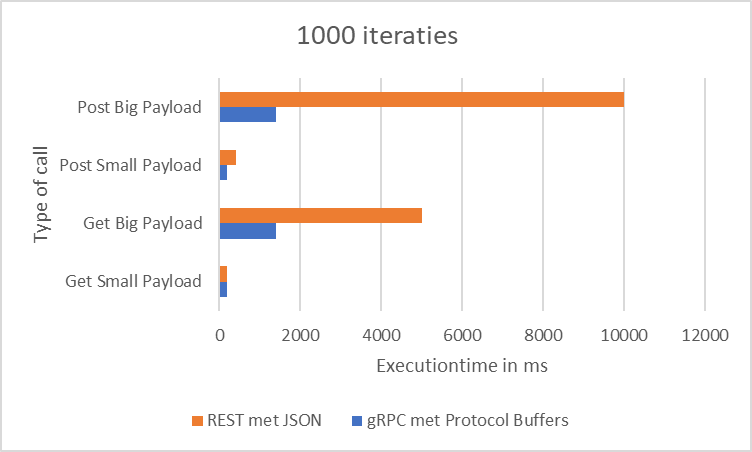
\includegraphics[width=1\linewidth]{screenshot001}



	\centering
	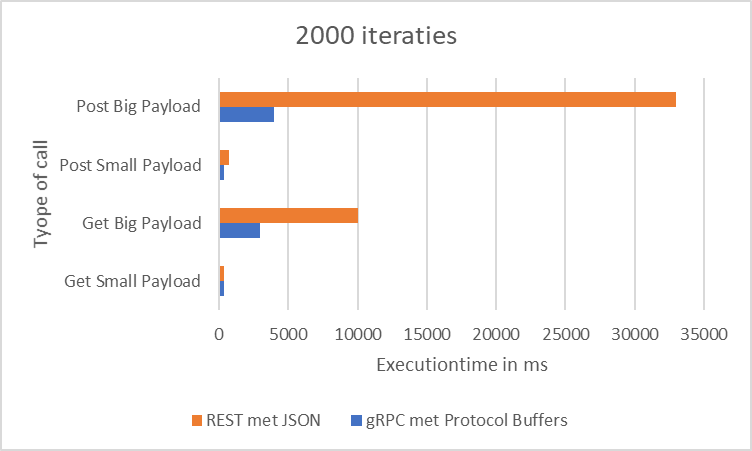
\includegraphics[width=1\linewidth]{screenshot002}

	



%---------- Verwachte conclusies ----------------------------------------------
\section{Verwachte conclusies}
\label{sec:verwachte_conclusies}

Dit onderzoek moet doen blijken of gRPC en Protocol Buffers sneller en efficiënter zijn dan een REST API met JSON. In de PoC zal duidelijk worden dat gRPC en Protocol Buffers een sneller en efficiënter alternatief zijn voor JSON. Dit resultaat zou eventueel verklaard kunnen worden doordat JSON een ouder dataformaat is en dus niet geoptimaliseerd is voor de huidige technologieën terwijl gRPC zeer recent ontworpen is om optimaal met de huidige technologieën om te gaan.



%%---------- Andere bijlagen --------------------------------------------------
% TODO: Voeg hier eventuele andere bijlagen toe
\chapter{Copyright Notice Ecma International}
"COPYRIGHT NOTICE
© 2017
Ecma International

This  document ~\autocite{Json2017}  may  be  copied,  published  and  distributed  to  others,  and  certain  derivative  works  of  it may  be  prepared,  copied,  published,  and  distributed,  in  whole  or  in  part,  provided  that  the  above copyright  notice  and  this  Copyright  License  and  Disclaimer  are  included  on  all  such  copies  and derivative  works.  
The  only  derivative  works  that  are  permissible  under  this  Copyright  License  and Disclaimer are: 

(i) works which incorporate all or portion of this document for the purpose of providing commentary or explanation (such as an annotated version of the document),

(ii)    works  which  incorporate  all  or  portion  of  this  document  for  the  purpose  of  incorporating  features that provide accessibility,

(iii)   translations of this document into languages other than English and into different formats and

(iv)    works  by  making  use  of  this  specification  in  standard  conformant  products  by  implementing  (e.g. by copy and paste wholly or partly) the functionality therein.

However, the content of this document itself may not be modified in any way, including by removing the copyright  notice  or  references  to  Ecma  International,  except  as  required  to  translate  it  into  languages other than English or into a different format.

The  official  version  of  an  Ecma  International  document  is  the  English  language  version  on  the  Ecma International  website.  In  the  event  of  discrepancies  between  a  translated  version  and  the  official version, the official version shall govern.

The limited permissions granted above are perpetual and will not be revoked by Ecma International or its successors or assigns.

This  document  and  the  information  contained  herein  is  provided  on  an  "AS  IS"  basis  and  ECMA INTERNATIONAL  DISCLAIMS  ALL  WARRANTIES,  EXPRESS  OR  IMPLIED,  INCLUDING  BUT  NOT LIMITED   TO   ANY   WARRANTY   THAT   THE   USE   OF   THE   INFORMATION   HEREIN   WILL   NOT INFRINGE ANY OWNERSHIP RIGHTS OR ANY IMPLIED WARRANTIES OF MERCHANTABILITY OR FITNESS FOR A PARTICULAR PURPOSE

%%---------- Referentielijst --------------------------------------------------

\printbibliography[heading=bibintoc]

\end{document}
